%
% File: chap02.tex
% Author: Oliver J. H. Feighan
% Description: delta-scf benchmarking, including dft and dftb methods.
% Talk about important factors for modelling LH2
%
%\let\textcircled=\pgftextcircled
\chapter{Mean-Field excited states}
\label{chap:dscf}

\subsubsection*{Previous Published Work}
Parts of the work presented in this chapter are also included in a paper published 
with Dr Susannah Bourne-Worster in March 2021\cite{Worster2021}. These sections
include parts of section \ref{sec:benchmarking} from \ref{subsec:reference_data}
up to but excluding \ref{subsec:dscf_gfn_tests}.

\initial {T}his chapter investigates the accuracy of \dscf methods with  both an 
ab initio DFT level of theory as well as with semi-empirical, tight-binding approximations.
\dscf is a well-known method for calculating transition energies, as well as
ionisation potentials, electron affinities and other properties. Although slightly
less accurate than other high-level response theories, it is much more efficient,
requiring only two SCF solutions for the two states involved in a transition. 

Whilst \dscf has been benchmarked against other methods in previous studies, it
has not been explicitly applied to chlorophyll systems in much detail before. It
is possible that this response method could be a good replacement for the more expensive
TD-DFT calculations used to obtain the response properties needed to make exciton
models. This would work best when generating training data for the statistical methods
discussed in section \ref{sec:stats_methods}, as these require a smaller volume
of calculation than a full time series of Hamiltonians.

For this second situation, the response method would still need to be as efficient
as the lightweight machine-learning or tight-binding methods. Here it is was investigated
whether these \dscf methods with tight-binding methods may solve this problem as
well. These are novel response methods, and so required benchmarking against high-level 
data to assess their abilities.

This approach to finding efficient response methods for LHCs would then follow a
similar pattern to that discussed in chapter \ref{chap:intro}. Using these more
efficient response methods to calculate transition properties, exciton Hamiltonians
could be constructed either for a relatively smaller set of geometries using DFT
based \dscf or for a relatively larger set using tight-binding based \dscf. This
is all dependent on their performance.

Transition properties were calculated for a range of molecules, as well as
for a small set of chlorophyll geometries, using variety of different basis sets,
density functionals, response methods and electronic structure methods. Most of 
the work was compared to either high-standard EOM-CCSD or SCS-CC2 reference to
draw conclusions on the accuracy of each method. Addressing the issue of non-orthogonality 
between the ground and excited states was also investigated for \dscf. Generally
it was found that the semi-empirical \dscf methods may not be applicable to LHC
models for reasons discussed in the following sections.

\section{Combining \dscf With Lower Level Electronic Structure Theories}
\label{sec:dscf_theory}
It is clear that the efficiency of \dscf methods could be increased by swapping out
the usual DFT electronic structure methods with a tight-binding or semi-empirical approach.
This would not cause any changes in the response method, only in the source of molecular
orbital coefficients used to construct the excited states. There are several frameworks 
that could have been chosen for this purpose, but the recently published GFN-xTB
method, parameterized by the Grimme group \cite{Grimme2017}, was ultimately used.
This method has been parameterized for geometries, frequencies and non-covalent 
interactions, and uses an extended version of H{\"u}ckel theory. The name GFN-xTB
is an acronym for "Geometries, Frequencies, Non-Covalent - eXtended Tight Binding".
This method was chosen as a similar response method that calculates transition 
properties, the sTDA-xTB method, also exists and is the precursor to the GFN-xTB methods.
Additionally the GFN-xTB method is implementated in many packages, including the
\code{QCORE} package, and this significantly reduces the amount of effort required to
implement and test. This became an important factor, necessary for the project 
discussed in the next chapter.

There are many forms of GFN-xTB, dependent on the level of theory of treated inter-electron
interactions, named GFN1-, GFN2- and GFN0-xTB. Due to considerations about the gradients 
of transition properties (discussed in the conclusion chapter), GFN2-xTB was not
included in this benchmarking. The method of using GFN1-xTB and GFN0-xTB electronic 
structure properties for \dscf transitions is referred to as \dxtb.

\section{Benchmarking \dscf}
\label{sec:benchmarking}
\subsection{Reference Data and test set}
\label{subsec:reference_data}
Full scale chlorophyll molecules are too large to be able to calculate a high-level
benchmark. It would not be possible to test \dscf data against coupled cluster data.
Instead a stepwise approach was used, covering a large chemical space by using a
range of molecules before focusing on niche systems. This range of molecules could
be smaller so high-level coupled cluster data could be generated.

A test set of small molecules, which would cover the same range of elements
as found in organic chromophores and biological molecules, was chosen as to benchmark 
both the \dscf methods as well as TD-DFT. The test set chosen was previously used
by the Grimme group to parameterise and test the sTDA-xTB method \cite{Grimme2017},
and as it was constructed to design new response methods it would contain a wide 
range of systems to appropriately benchmark the \dscf methods.

The test set consisted of 109 small molecules. Each system was closed-shell, 
contained 12 atoms or less, and contained on H, C, N, O and F atoms. The three lowest
energy singlet excited state transition energies were calculated using EOM-CCSD
with an aug-cc-pVTZ basis set. These results were generated using the Gaussian 16 
program \cite{Gaussian16}.

\subsection{Small Systems}
\label{subsec:smalltest}
Transition properties for this test set were calculated using TD-DFT and \dscf,
both using a CAM-B3LYP functional and aug-cc-pVTZ basis set. The transitions were
assigned to the EOM-CCSD results by comparing transition dipoles, energies and 
the character of the MOs involved in the transitions. Symmetry assignments were
also used where possible, but this was not the case for all systems either due to
unsuccessful labelling or defaulting to a non-Abelain group. Symmetry labelling 
was also only available for TD-DFT calculations, as these were performed with Gaussian
16. \dscf calculations were done with the \code{QCORE} program.

As the \dscf singlet transition is not a correct representation of a true singlet
excitation, which is a superposition of both spin-conserving $\alpha \rightarrow a,
\alpha$ and spin-flipping $\alpha \rightarrow a, \beta$ excitations, the spin-purification 
formula:

\begin{equation}
\Delta E_S = 2\Delta E^{i,\alpha \rightarrow a, \alpha} - \Delta E^{i,\alpha \rightarrow a, \beta}
\end{equation}
%
was used to correct for the true singlet excitation energy $\Delta E_S$ \cite{Ziegler1977}.

The results of comparing transition energies and transition dipole magnitudes are
shown in figures \ref{fig:energy_scatter} and \ref{fig:dipole_scatter}.

\begin{figure}
\centering
\includegraphics[scale=0.6]{../../Year_3/dscf_figures/energy_scatter.png}
\caption{Transition energies $\Delta E$ from TD-DFT (black) and \dscf (red)
 plotted against EOM-CCSD energies, with the line $y=x$ (dashed) for reference.
 The ethene dimer outlier has been circled.}
\label{fig:energy_scatter}
\end{figure}

\begin{figure}
\centering
\includegraphics[scale=0.6]{../../Year_3/dscf_figures/dipole_scatter.png}
\caption{Transition dipole magnitudes from TD-DFT (black) and \dscf (red) plotted
against EOM-CCSD transition dipole magnitudes, with the line $y=x$ (dashed) for 
reference.}
\label{fig:dipole_scatter}
\end{figure}

Overall, the excitation energies calculated with \dscf are as accurate at predicting
EOM-CCSD energies as TD-DFT. The mean error is 0.35 eV, with a standard deviation
of 0.25 eV. This is a marginal improvement on the TD-DFT results, which has a mean
and standard deviation of 0.41 eV and 0.27 eV respectively. Transition dipoles 
were similarly accurate to the reference data, although \dscf performs slightly 
worse in this respect. The mean and standard deviation in the absolute value
of transition dipole moment, $|\mathbf{\mu}|$, was 0.07 a.u. and 0.08 a.u. respectively.
For TD-DFT, the mean and standard deviation were 0.03 a.u. and 0.06 a.u. (the atomic
unit here being equal to $ea_0$).
The outlier circled in figure \ref{fig:energy_scatter} is an ethene dimer system,
and shows the inability of \dscf to capture a mixed excited state. The two LUMO
orbitals in this dimer system include in-phase and out-of-phase combinations of the 
$\pi$-antibonding orbitals, and are very close in energy. The HOMO orbitals are
the same on both ethene molecules, being the $\pi$-bonding orbitals, which are
degenerate in energy. The first excited state is predicted by TD-DFT and EOM-CCSD
to be a mix of these two close HOMO-LUMO transitions. However \dscf cannot include
this mixed behaviour as it only considers single transitions. \dscf predicts two
transition energies of 7 eV and 10 eV, whilst TD-DFT and EOM-CCSD predict 7.5 eV.
The outlier in figure \ref{fig:dipole_scatter} is due to \dscf finding a different
but still valid description of the transition dipole for a stretched benzene system,
where the HOMO-1, HOMO, LUMO and LUMO+1 orbitals are all degenerate. The \dscf transition
dipole magnitude agrees with the value of an equally mixed HOMO - LUMO+1 and HOMO-1 
- LUMO transition, which given the degeneracy is an equally valid description of 
the transition.

In summary, \dscf can be seen to accurately predict transition properties
to a EOM-CCSD level of accuracy with as much success as TD-DFT, except in cases
of mixed transitions. 

\subsection{Non-orthogonality}
\label{subsec:dscf_nonorth}
Generally the ground and excited states calculated for \dscf transition, being solutions
from two separate SCF cycles, will not be completely orthogonal. The Slater determinants
$\ket{\Psi_n}$, are constructed from a set of mutually orthogonal orbitals $\{ \ket{\phi_j^{\left(n\right)}} \}$,
such that orbitals will be orthogonal within the same state. However there is no 
orthogonality constraint on sets of orbitals derived from independent SCF cycles
so it is possible for the overall states $\Psi_1$ and $\Psi_2$ to overlap such 
that the inner product,

\begin{equation}
S^{21}_{jk} = \braket{\phi_j^{\left(2\right)} | \phi_k^{\left(1\right)}}
\end{equation}
%
will be non-zero. Similarly, there will be a non-zero transition charge,

\begin{equation}
q^{21} = \braket{\Psi^2|\Psi^2}
\end{equation}
%
, which breaks the origin-independence property of the transition dipole moment. In
this way, any transition dipoles that do not have their centre at the origin will
have a systematic error based on this overlap and the distance from the origin.
For vertical transitions, this transition charge should be zero, and so all transition
dipole moments calculated with non-orthogonal \dscf would always have this error.

In order to fix this issue, the standard transformation to symmetrically orthogonalise 
the two states was applied, which also would preserve as much character of the 
original states as possible. The transformation is given by

\begin{equation}
\ket{\Psi_{\tilde{\nu}}} = \sum_{\nu} \ket{\Psi_\nu} \left[\mathbf{S}^{-\frac{1}{2}} \right]_{\nu\tilde{\nu}}
\end{equation}
%
where $\mathbf{S}$ here is a block matrix

\begin{equation}
\mathbf{S} = \begin{pmatrix}
    1 & S \\
    S & 1 
\end{pmatrix}
\end{equation}
%
with $S$ being the overlap value of the two states $\braket{\Psi_2|\Psi_1}$.

\begin{figure}
\centering
\includegraphics[scale=0.6]{../../Year_3/dscf_figures/correction_scatter.png}
\label{fig:correction_scatter}
\caption{The absolute value of the error in transition dipole magnitude between
\dscf and EOM-CCSD, plotted against the \dscf overlap of the ground and excited
state. All systems were translated by 100 \AA{} in all cartesian axes. Transition
dipole magnitudes calculated without any correction are shown in red, whilst
those with the symmetric orthogonalisation correction are shown in black.}
\end{figure}

It was found that using this method for correcting the non-zero overlap of states, 
the origin-independence of the transition dipole moment was recovered (see figure
\ref{fig:correction_scatter}).
The transition dipole for each molecule in the test set systems was calculated
for molecules translated by 100\AA{} in the $xyz$ direction.
This would induce an error for the non-orthogonalised states, which was corrected 
by symmetric orothogonalistion. It should be noted that whilst this effect is dependent
on how large the overlap may be, and it could be argued that with a small overlap 
this effect may not be large, having any large translation of the molecule (on the order of hundreds of angstroms) 
can be seen to lead to completely incorrect transition dipole magnitudes. In a
large protein system, where chromophores can easily be tens or hundreds of angstrom
from the overall system origin, this would obviously present a much larger problem 
than for a vacuum-phase small molecule.

\subsection{LH2 Chlorophyll}
\label{subsec:dscf_chl_tests}
Having demonstrated that TD-DFT is a good proxy for high-level methods, \dscf was
benchmarked against TD-DFT data for a series of chlorophyll molecules. This would
show how well \dscf methods could be used in simulating a whole LH2 system.

The PBE0 functional with Def2-SVP basis set \cite{Adamo1999, Schafer1992} was used
to calculate both TD-DFT and \dscf properties. This has been used previously for 
BChla structures, and has been shown to be a good balance between accuracy and cost 
\cite{Stross2016}. 

\begin{figure}
\centering
\includegraphics[scale=0.6]{../../Year_3/dscf_figures/chlorophyll_energy_scatter.png}
\label{fig:chl_energy}
\caption{Transition energies from \dscf for 26 chlorophyll geometries from the LH2
protein of purple bacteria,  plotted against energies from TD-DFT. The line of
best fit ($R^2=0.87$) is shown as the dashed line. Both methods used a PBE0/Def2-SVP 
level of theory.}
\end{figure}

\begin{figure}
\centering
\includegraphics[scale=0.6]{../../Year_3/dscf_figures/chlorophyll_dipole_scatter.png}
\caption{Transition dipole magnitudes from \dscf for the same 26 chlorophyll geometries as
\ref{fig:chl_energy}, plotted against dipole magnitudes from TD-DFT. The line of
best fit ($R^2= 0.57$) is shown as the dashed line. Both methods used a PBE0/Def2-SVP
level of theory.}
\label{fig:chl_dipole}
\end{figure}

The high degree of correlation between \dscf and the TD-DFT results demonstrates
that the variations in transition energies are due to differences in geometry, rather
than any noise from random error. The systematic error is expected, and all methods
used would have an associated error that is usually removed by a constant parameter.

The error in transition dipole magnitudes is larger than that of the small
test set. This error is about 0.42 a.u. larger, but without EOM-CCSD or another
high-level method, it's unclear whether this error might be from TD-DFT or \dscf.
Additionally, there is a clear correlation between the transition dipole magnitudes
from TD-DFT and \dscf, and so whilst quantitative results would not be possible, 
qualitative statements could be made from \dscf data. For example, whilst the exact 
value of a transition dipole moment at a given geometry may not be accurate, the
change in transition dipole moment from several geometries would be similar in
variation to TD-DFT calculated properties.

An important point to take note of is that it was not possible to calculated the 
excited state for all 27 chlorophyll geometries, as one geometry repeatedly collapsed back
down to the ground state. Methods such as including previous iterations' Fock matrices
into the current Fock matrix (i.e. Fock damping), using intermediate initial guesses like 
half-electron promotions, and alternative DIIS procedures, had little effect on 
improving this collapse. Other methods could have been tried, such as the initial
maximum overlap method (iMOM), where the projection in the MOM procedure is based 
on one static set of orbitals rather than the previous SCF cycle, but implementing
and testing these methods is outside the scope of this work.

\afterpartskip
\subsection{xTB methods}
\label{subsec:dscf_gfn_tests}
\dxtb was tested on the same small molecule benchmark set. It's performance was 
compared to other methods with a range of approximations for calculating transition
properties, including a proxy for sTDA-xTB results. To include this in the comparison
it was necessary to use spin-component-scaled second order coupled-cluster (SCS-CC2)
\cite{Hattig2000, Hellweg2008} reference data produced by Grimme et al. \cite{Grimme}.
Two types of \dxtb were investigated, based on GFN1-xTB and GFN0-xTB properties.
GFN0-xTB is similar to the GFN1-xTB method, but excludes any charge dependent terms
in its Fock matrix so is not self-consistent. Therefore only a single diagonalisation
is necessary for GFN0-xTB, and the same molecular orbital coefficients are used for
ground and excited state. A transition energy from \dscf with this method would
functionally be the same as an eigenvalue difference.
The eigenvalue differences from sTDA-xTB, given by the \code{xtb4stda} program
\cite{Grimme2016}, were also included in this benchmarking. This was done to observe
whether the electronic structure or the response method is more important in achieving
accuracy with the sTDA-xTB method. This was done with the \code{xtb4stda} program,
the first of two programs that runs a version of xTB which provides molecular orbital
coefficients and energies for the sTDA program to use to calculate the transition
properties.

The full list of methods included in the comparison is:
\begin{itemize}
    \item High level TD-DFT, with a range separated functional CAM-B3LYP and
     a aug-cc-pVTZ basis set.
    \item Lower level TD-DFT, with a PBE0 functional and smaller Def2-SVP basis set.
    \item \dscf with CAM-B3LYP/aug-cc-pVTZ.
    \item \dscf with PBE0/Def2-SVP.
    \item linear response with GFN1-xTB and GFN0-xTB.
    \item \dscf with GFN1-xTB and GFN0-xTB, named \dxtb.
    \item Full sTDA-xTB.
    \item sTDA-xTB eigenvalue difference.
\end{itemize}
 
\subsubsection{Post-SCF Assignment of Symmetry}
\label{subsubsec:post_scf_symmetry}

A source of error that hasn't been discussed in much detail so far is the assignment
of transitions between different methods. A known problem of \dscf methods is that
the excited state SCF cycle may not converge to the correct state, or it might
collapse back to the ground state. This could be seen in the symmetry of the excitation
- if \dscf has converged to a different transition than TD-DFT and CC2, the symmetry 
label of transition would also be different. The benchmarking discussed previously
used symmetry labels to assign TD-DFT transitions to EOM-CCSD but as noted earlier
this was not always possible, and assigning symmetry labels to \dscf was not possible.
Instead, transition dipole orientations and plots of MOs were used. Whilst a possible
approach for \dxtb, the difference between \dxtb valence basis sets and full DFT
basis sets caused issues. Instead the issue of assigning symmetry to \dscf transitions
was investigated in more detail.

Assigning symmetry to \dscf transitions would require assigning symmetry to both
molecular orbtials and the overall wave-function of a molecule. Most electronic 
structure codes have two choices in assigning symmetry to orbitals - either all
of the SCF code will treat symmetry from the outset, or nothing is assigned in the
SCF code and assignment will happen post-SCF. Both these approaches have benefits
and drawbacks.

The first method means the symmetry to be known at any point in the SCF procedure,
and allows the Hamiltonian to be organized into a block matrix which is more efficient
to diagonalise. This can be especially useful when solving for a large basis set 
or large system, as the matrix diagonalisation can be partitioned and parallelised 
over several cores or nodes on a cluster computer. However this works best if the
system is highly symmetric, which is often only the case when treating optimized 
systems. This discounts systems from molecular dynamics simulations as well as many
biological systems.

The second approach of assigning symmetry after the SCF cycles does not fix these
drawbacks but it does allow for codes which originally didn't have symmetry assignment
to be used without rewriting SCF code. The obvious drawback of doing assignment 
post-SCF is that symmetry can't be utilized during the SCF procedure.

The symmetry label of an orbital is given by the character of that orbital in symmetry
subspaces of the point group of the system. These characters are calculated by transforming
the molecular orbital coefficients $\mathbf{C}$ into each subspace $A$ by using
the transformation matrix $\mathbf{T}$, defined by

\begin{equation}
\tilde{\mathbf{C}}_A = \mathbf{T}^T_A \mathbf{S} \mathbf{C}
\end{equation}
%
, and then summing the coefficients to obtain the character

\begin{equation}
P_A = \sum_{\nu} \left\lvert \tilde{\mathbf{C}}_{A, \mu\nu} \right\rvert
\end{equation}
%
, where $\mu,\nu$ are indices for the atomic and molecular orbitals respectively. 
The molecular orbital with character equal to 1 in a subspace would then have that
symmetry label, and would be a well defined assignment. However, in practice this was
not always clear cut and so the highest subspace character was taken as the assignment.

The steps for assigning orbital symmetry post-SCF is as follows:

\begin{enumerate}
    \item Determine the point group of the molecule, from the atomic positions. This
    determines the symmetry subspaces.
    \item Get the symmetry adapted linear combinations (SALCs) of atomic orbitals for 
    each subspace.
    \item Use the SALCs to construct the transformation matrix $T$ that will .
    \item Assign the one electron molecular orbital (MO) for these subspace characters
     with the symmetry adapted linear combinations.
    \item Multiply the one electron MO symmetries together to find the symmetry 
    of the overall wavefunction.
\end{enumerate}

\begin{figure}
    \centering
    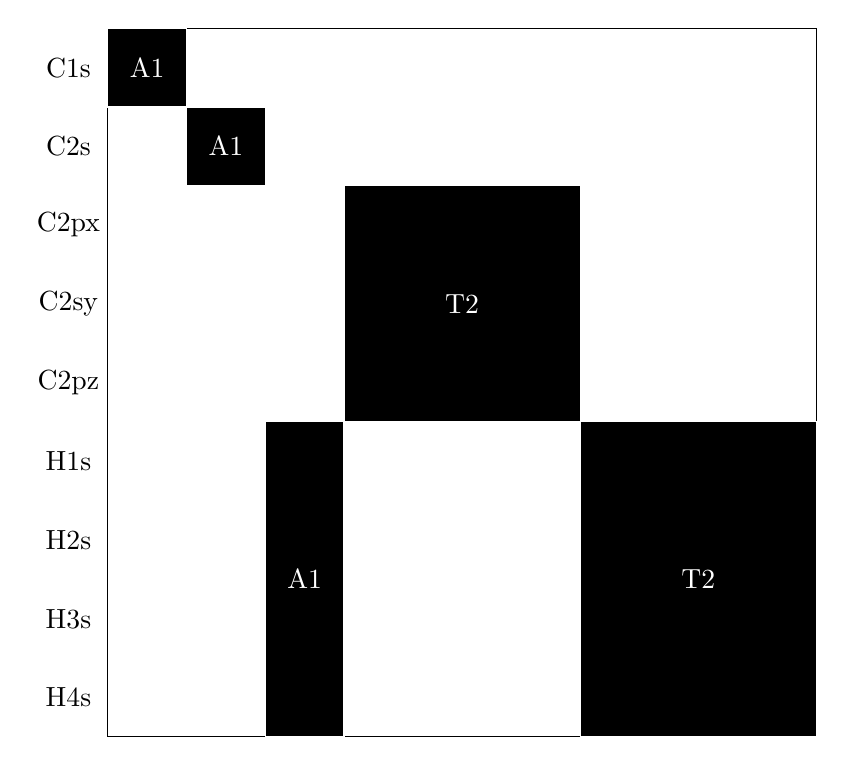
\begin{tikzpicture}
        \node[draw=none,
        rectangle, 
        minimum width = 1cm, 
        minimum height = 1cm
        ](r) at (-5cm,4cm) {C1s};
        \node[draw=none,
        rectangle, 
        minimum width = 1cm, 
        minimum height = 1cm
        ](r) at (-5cm,3cm) {C2s};
        \node[draw=none,
        rectangle, 
        minimum width = 1cm, 
        minimum height = 1cm
        ](r) at (-5cm,2cm) {C2px};
        \node[draw=none,
        rectangle, 
        minimum width = 1cm, 
        minimum height = 1cm
        ](r) at (-5cm,1cm) {C2sy};
        \node[draw=none,
        rectangle, 
        minimum width = 1cm, 
        minimum height = 1cm
        ](r) at (-5cm,0cm) {C2pz};
        \node[draw=none,
        rectangle, 
        minimum width = 1cm, 
        minimum height = 1cm
        ](r) at (-5cm,-1cm) {H1s};
        \node[draw=none,
        rectangle, 
        minimum width = 1cm, 
        minimum height = 1cm
        ](r) at (-5cm,-2cm) {H2s};
        \node[draw=none,
        rectangle, 
        minimum width = 1cm, 
        minimum height = 1cm
        ](r) at (-5cm,-3cm) {H3s};
        \node[draw=none,
        rectangle, 
        minimum width = 1cm, 
        minimum height = 1cm
        ](r) at (-5cm,-4cm) {H4s};
        
        \node[draw,
        rectangle, 
        minimum width = 9cm, 
        minimum height = 9cm
        ](r) at (0cm,0cm) {};

        \node[draw,
        rectangle, 
        color=white,
        fill=black,
        minimum width = 1cm, 
        minimum height = 1cm
        ](r) at (-4cm,4cm) {A1};

        \node[draw,
        rectangle,
        color=white, 
        fill=black,
        minimum width = 1cm, 
        minimum height = 1cm
        ](r) at (-3cm,3cm) {A1};

        \node[draw,
        rectangle,
        color=white,
        fill=black,
        minimum width = 1cm, 
        minimum height = 4cm
        ](r) at (-2cm,-2.5cm) {A1};

        \node[draw,
        rectangle, 
        color=white,
        fill=black,
        minimum width = 3cm, 
        minimum height = 3cm
        ](r) at (0cm,1cm) {T2};

        \node[draw,
        rectangle, 
        color=white,
        fill=black,
        minimum width = 3cm, 
        minimum height = 4cm
        ](r) at (3cm,-2.5cm) {T2};

    \end{tikzpicture}
    \label{fig:methane_symmetry}
    \caption{A breakdown of the symmetry orbitals in STO-3G methane into the subspaces 
    present in the T\textsubscript{d} point group.}
\end{figure}

This procedure was implemented and tested on methane with a minimal STO-3G basis set,
using the open source library libmsym \cite{libmsym} for point group assignment
functions and finding SALCs. The MOs for an optimised methane geometry with an STO-3G 
basis set were correctly assigned using this method (two occupied orbitals and one
unoccupied orbital of A1 symmetry, and three occupied and unoccupied orbitals of 
T2 symmetry). A diagrammatic representation of the subspace characters of molecular
orbitals is shown in figure \ref{fig:methane_symmetry}. The overall wavefunction
symmetry can then be expressed as the product of all MO symmetries, reduced with
the reduction formula

\begin{equation}
n = \frac{1}{h} \sum_R \xi_r \left( R \right) \xi_i \left( R \right)
\end{equation}
%
, where $\xi_r, \xi_i$ are the reducible and irreducible representations respectively,
$h$ is the order of the group and $R$ is the subspace. This correctly produced
the overall symmetries of ground state systems for methane, as well as water.

Generally the subspace characters were binary for these easy test cases, however 
MOs of excited states were found to be mixed, making any assignment unclear for
many MOs. This was also the case for non-abelian groups, where there would be degenerate
subspaces. This is similar to the problem of assigning symmetry for the TD-DFT and
EOM-CCSD transitions in the earlier benchmarking. Often this caused reduction of ground
state wavefunctions to give non-physical answers.

Overall while improving some features of \dscf methods is in the scope of this project,
this type of assignment is flawed for LH2 system. Although it would be a useful 
feature for the benchmarking test-sets, chlorophyll molecules would be far from
symmetric and so this type of assignment could not have been expected to have worked.
Ultimately transitions could not be confidently assigned for \dscf with this method.
Hence while careful consideration was made for this problem, benchmarking of the
\dxtb methods could be expected to still have some errors associated to this issue.
In the end the assignment of symmetry was based on the previously used inspection
of transition dipole orientations and transition density plots.

\subsubsection{\dxtb Benchmarking Results}
\label{subsubsec:imp_of_benchmarking}

The distributions of errors to SCS-CC2 data for each of the benchmarking methods,
as well as a generated distribution of sTDA-xTB results, are shown in figure \ref{fig:dxtb_absolute_errors}.
The means and standard deviations are reported in table \ref{table:mean_std_devs}.

\begin{figure}
    \centering
    \includegraphics[scale=0.6]{../../Year_2/test_sets/sTDA_xtb_fit/stda_fit/HCNOF/dxtb_absolute_errors.png}
    \caption{The distributions of errors compared to SCS-CC2 transition energies for the methods
    included in the \dxtb benchmarking.}
    \label{fig:dxtb_absolute_errors}
\end{figure}

\begin{table}
\centering
\begin{tabular}{||c c c||}
    \hline
    Method & Mean / eV & Standard Deviation / eV \\ [0.5ex]
    \hline\hline
    TD-DFT CAM-B3LYP/aug-cc-pVTZ & -0.18 & 0.34 \\
    TD-DFT PBE0/Def2-SVP         & -0.06 & 0.79 \\
    \dscf CAM-B3LYP/aug-cc-pVTZ  & -0.14 & 0.28 \\
    \dscf PBE0/Def2-SVP          & -0.62 & 0.50 \\ 
    TD-GFN1-xTB                  &  0.27 & 1.47 \\ 
    TD-GFN0-xTB                  & -0.41 & 1.32 \\ 
    \dscf GFN1-xTB               & -0.12 & 2.11 \\ 
    \dscf GFN0-xTB               & -1.50 & 1.08 \\
    \code{xtb4stda}              &  4.39 & 1.26 \\  [1ex]
    \hline 
\end{tabular}
\caption{Mean and standard deviations of the errors, in eV, against SCS-CC2
reference data. The \code{xtb4stda} entry represents the eigenvalue difference
method that uses the eigenvalues output from this program.}
\label{table:mean_std_devs}
\end{table}

Overall, both \dxtb methods are inaccurate - far too inaccurate to be used as a 
viable method for transition properties of chlorophyll, or any other system.
The mean error GFN1-\dxtb was -0.12 eV, and has a significant standard deviation
of 2.11 eV. GFN0-\dxtb hd a larger mean error of -1.50 eV, and whilst a slightly
smaller standard deviation of 1.08 eV, this is still well beyond a usable accuracy.

The DFT methods, both the linear response and the \dscf methods, are still shown
to be accurate at predicting excitation energies, with means and standard deviations
within ranges previously reported in the above sections.

Due to these results it is argued that decreasing the level of theory for the electronic
structure dramatically decreases the accuracy of transition properties.
The highest level electronic structure method has the best accuracy. CAM-B3LYP/aug-cc-pVTZ 
TD-DFT and \dscf have mean errors of -0.18 eV and -0.14 eV and standard
deviations of 0.34 and 0.28 eV respectively. Both methods are well within the accuracy
needed to predict geometry-based variations. The outliers in the \dscf results are known 
mixed transitions, as discussed earlier with the ethene dimer system. 
The lower level PBE0/Def2-SVP methods have a marked decrease in accuracy. On going
from higher-level DFT to lower level, the standard deviation approximately doubles 
for both TD-DFT (0.34 eV to 0.79 eV) and \dscf (0.28 eV to 0.50 eV). Again, the
PBE0/Def2-SVP TD-DFT and \dscf are comparable, with standard deviations of 0.79 eV
and 0.59 eV, although the mean for \dscf has a significant shift of -0.62 eV. 

Comparing the DFT and GFN based methods, we can see the same trend that lowering
the level of theory gives worse transition properties.
Overall, the most inaccurate method is the eigenvalue difference methods based
orbital energies (eigenvalues of the Hamiltonian diagonalisation) from the \code{xtb4stda}
method. The means and standard deviation was 4.39 eV and 1.26 eV respectively,
a huge difference to the values for values for full sTDA-xTB (-0.04 eV and 0.41 eV respectively)\cite{Grimme2016}. 
Arguably then the sTDA method, and not the underlying xTB method, can make up a 
large part of the accuracy for predicting transition properties. A similar response 
theory then might be expected to perform equally well, which is investigated in 
more detail in the next chapter.

The result that GFN-xTB based methods are not accurate is not unexpected. As opposed
other DFT methods, which use \emph{ab initio} or first principle parameters, the
xTB methods were fit to target properties and so would not be expected to be suitable
for other properties outside the training data \cite{Bannwarth2020}. Whilst the 
lack of pair-wise parameters and "top-down" parameterisation approach which gives
GFN-xTB a better number and specificity of parameters compared to other methods, 
these parameters only extend the accuracy of predicted properties to different
chemical systems and not to different properties altogether.

\section{Conclusions}
\label{sec:dxtb_conclusions}
The transition properties of a test set of small molecules has been benchmarked 
with multiple \dscf, TD-DFT and high-level methods. It has been shown that DFT 
based \dscf and TD-DFT methods can reproduce the same transition energies and 
transition dipole magnitudes as EOM-CCSD to within reasonable levels
of accuracy. For the set of small molecules, transition energies were predicted
with a mean of less than 0.5 eV, and 0.07 a.u. for transition dipole magnitudes.
Additionally, the issue of breaking the origin independence property of transition
dipoles has been shown to be fixed by using a symmetric orthogonalisation of the 
two originally non-orthogonal states.

For a small set of BChla geometries, it was found that the same level of accuracy
for transition energy could be found between \dscf and TD-DFT, where EOM-CCSD was
too expensive to calculate. The error was well within the range of TD-DFT energy
variation, shown in the high correlation coefficient, and so \dscf could be reasonably
expected to give correct geometry-dependent transition energies. Whilst the accuracy
is slightly reduced for transition dipole moments, the appreciable degree of correlation
implies that qualitative statements would be valid.

With all of the above benchmarking, reliably obtaining and assigning transitions
predicted from \dscf has proved to be an unsolved issue. Either \dscf is formally
unable to predict the correct character of transitions, as showcased in the ethene 
dimer mixed transition outlier, or it is unreliable in finding excited state solutions.
This is best shown in the exclusion of a geometry of chlorophyll that could not
be made to converge to the correct excited state.

To solve the inability of currently implemented \dscf to assign symmetry labels,
a post-SCF method of assigning MO and full wavefunction symmetry was investigated,
but ultimately proved beyond the scope of this project. Whilst able to assign labels
for small, trivial systems of STO-3G water and methane, non-trivial excited states
and more complex systems did not work. Whilst there is more work that could be done
in this area, it was decided that this should be moved to potential further work
on \dscf methods.

GFN-xTB based methods, named \dxtb were found to be inaccurate to the point where
it they would not be a useful proxy to higher level methods. Due to the similarity
in results for linear response and \dscf methods over a range of electronic structure
methods this drop in accuracy is attributed to the different electronic structure 
theory rather than the response method. This implies that altering the electronic
structure method could lead to great improvements in the accuracy of a new response 
method.

The aim of this chapter was to determine whether \dscf methods, which have a simple
gradient theory and are less costly than TD-DFT, could provide a sufficiently accurate
description of transition properties for use in an \emph{ab initio} exciton framework.
It has been shown that this is true with the condition that the underlying theory
is sufficiently high. However there is still the outstanding issue for calculating
properties for a large volume of  chlorophyll structures. The efficiency of DFT calculations 
may be too low for a large exciton framework or for large monomer systems like Bchla.
Semi-emperical \dscf methods, which would be efficient enough, prove innaccurate 
in their current form. However, it is demonstrated that a correct electronic structure
and a "top-down" parameterisation could make an accurate semi-emperical method, 
which is investigated in the following chapter.
